\documentclass{article}
\usepackage{amsmath}
\usepackage{graphicx}
\usepackage{float}
\usepackage{geometry}
\usepackage{hyperref}
\usepackage{calc}
\usepackage{enumitem}
\usepackage{color}
\usepackage{adjustbox}
\usepackage{xcolor}
\hypersetup{
    colorlinks,
    linkcolor={red!50!black},
    citecolor={blue!50!black},
    urlcolor={blue!80!black}
}
\usepackage{xepersian}
\settextfont[
    Scale = 1.3 ,
    BoldFont = *Bd ,
    ItalicFont = *It ,
    Extension = .ttf
]{XB Niloofar}
\AddEnumerateCounter{\alph}{\@alph}{\faalph}

\geometry{
    left=20mm,
    right=20mm,
    top=20mm,
    bottom=20mm,
}


\begin{document}
\begin{titlepage}
    \begin{center}
        \textbf{\Huge{گزارش آزمایش پنجم آزمایشگاه
        \\ طراحی سیستم دیجیتال}}\\
        \vspace{1cm}
        
\includegraphics[width=0.3\textwidth]{sharif.jpg}\\
        \vspace{1cm}
        \textbf{ \Large{مزدک تیموریان}}\\
        \vspace{0.4cm}
        \textbf{ \large{401101495}}\\
        \vspace{0.5cm}
        \textbf{ \Large{مریم شیران}}\\
        \vspace{0.4cm}
        \textbf{ \large{400109446}}\\
        \vspace{0.5cm}
        \textbf{ \Large{مهدی بهرامیان}}\\
        \vspace{0.4cm}
        \textbf{ \large{401171593}}\\
        \vspace{1cm}
        \textbf{ \Large{دانشکده مهندسی کامپیوتر}}\\
        \vspace{0.4cm}
        \textbf{ \Large{دانشگاه صنعتی شریف}}\\
        \vspace{0.6cm}
        \large{تیر 1403}
    \end{center}
    \thispagestyle{empty}
\end{titlepage}

\tableofcontents

\newpage

\section{مقدمه}
هدف از اين آزمايش طراحی یک واحد ضرب كننده است كه برای انجام عمل ضرب از روش ضرب
Booth
استفاده میکند.
برای انجام این آزمايش 
مسيرداده و واحد كنترل را جداگانه طراحی
کرده و سپس آنها را بهم متصل میکنیم.

\begin{figure}[H]
    \centering
    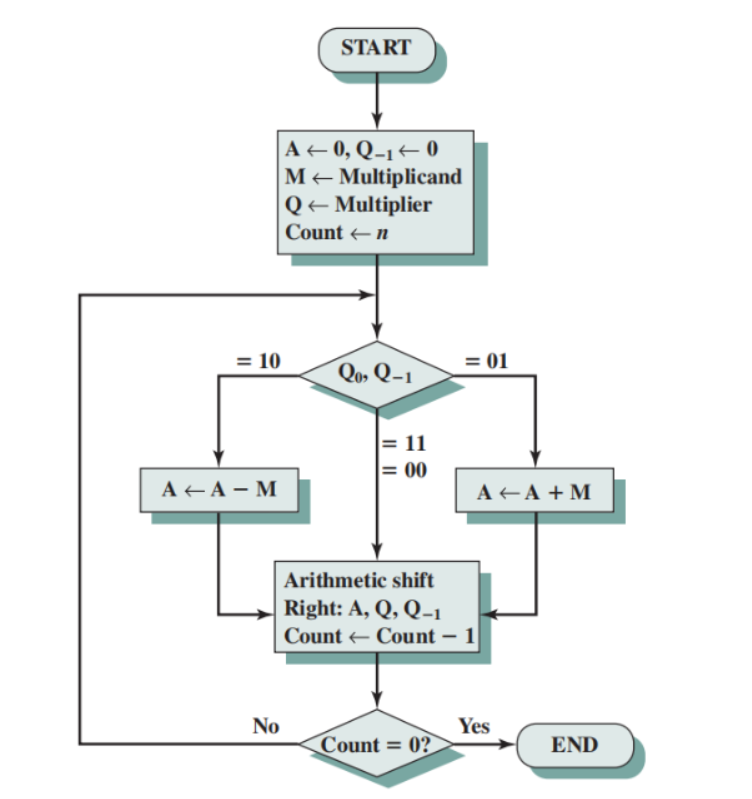
\includegraphics[width=\textwidth]{BF.png}
\end{figure}

نمودار الگوریتم 
Booth 
را نیز میتوانید در شکل بالا مشاهده کنید 
که با شیفت دادن یک عدد و چک کردن تغییر بیت از 0 به 1 و یا بالعکس مقدار عدد
دوم را از حاصل کم کرده و یا به آن اضافه میکند.

\section{شرح آزمایش}

\subsection{\LR{First Indices}}
برای اینکه عملیات شیفت به راست سریع‌تر انجام شود بیت‌های تکراری 
0 و 1 را شناسایی کرده و در یک کلاک به تعداد آنها شیفت میدهیم زیرا
در آن حالت جمع و یا تفریقی انجام نمیشود.

برای انجام این کار ماژولی طراحی میکنیم که اولین بیت 0 و 1 را در عدد پیدا کند.

\begin{figure}[H]
    \centering
    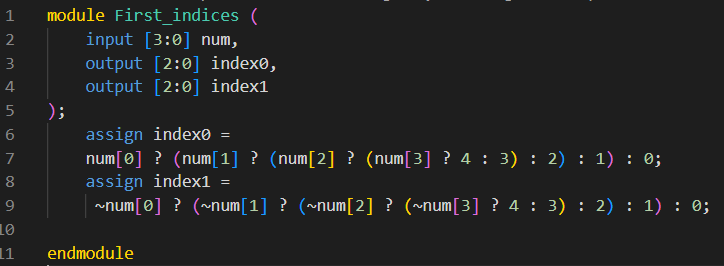
\includegraphics[width=0.8\textwidth]{FI.png}
\end{figure}

همچنین برای بررسی درستی آن ماژول تست زیر را طراحی کرده‌ایم.

\begin{figure}[H]
    \centering
    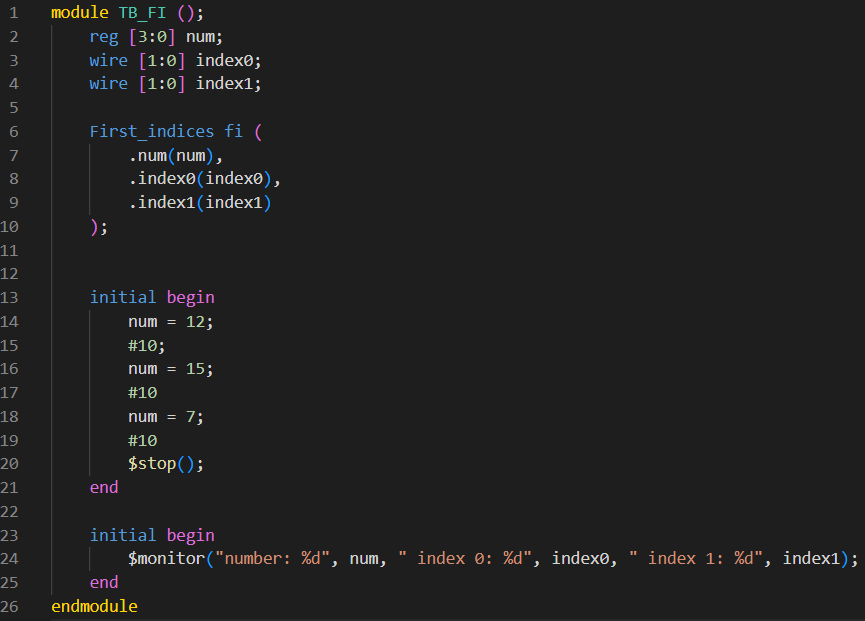
\includegraphics[width=0.8\textwidth]{TB_FI.png}
\end{figure}
\newpage
\subsection{Datapath}

در ادامه مسیر داده را طراحی میکنیم.
\begin{figure}[H]
    \centering
    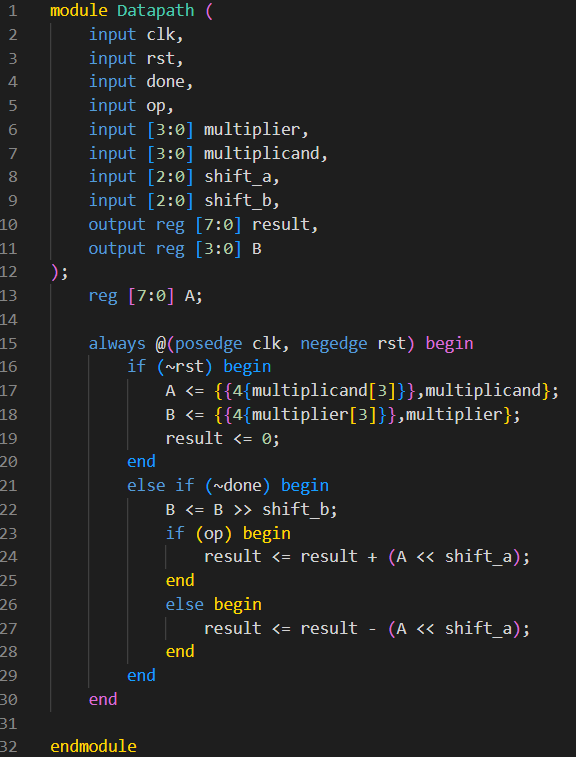
\includegraphics[width=0.95\textwidth]{DP.png}
\end{figure}
همانطور که در شکل بالا مشاهده میکنید در شروع برنامه ابتدا 
multiplicand 
و
multiplier
را 
\LR{Sign Extend}
کرده و در 
A
و
B
میریزیم.
سپس در هر مرحله 
B
را به راست شیفت داده و بجای شیفت دادن 
result
(نتیجه ضرب)
عدد 
A
را به چپ شیفت داده و با توجه به مقدار
op
که از روی 
01 و یا 10 بودن
دو بیت سمت چپ معلوم میشود مقدار حاصله را با 
result
جمع کرده و یا از آن کم میکنیم.
این پروسه را تاجایی ادامه میدهیم که واحد کنترلی سیگنال 
done 
را 1 کند که به معنای آماده شدن نتیجه است.

\newpage
\subsection{\LR{Control Unit}}

حال واحد کنترلی را طراحی میکنیم که وظیفه آن مشخص کردن سیگنال‌های 
کنترلی از روی وضعیت مدار است.

\begin{figure}[H]
    \centering
    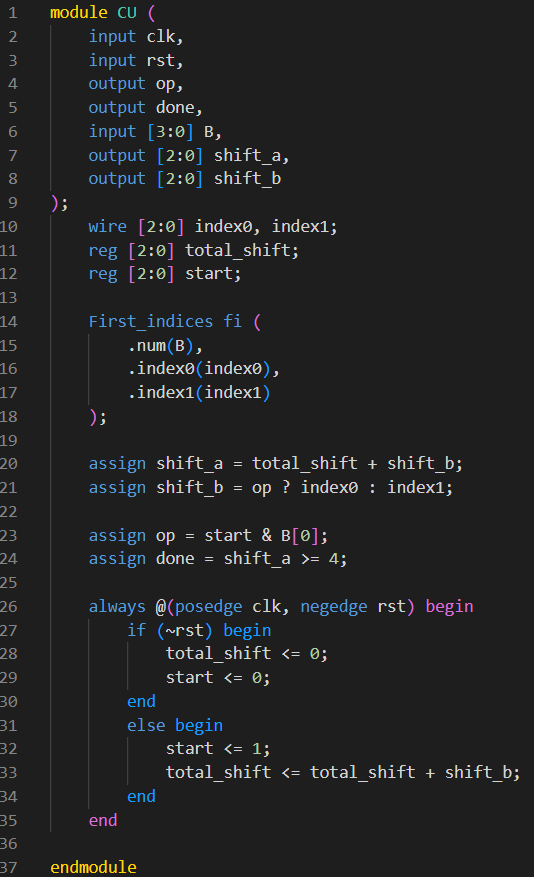
\includegraphics[width=0.75\textwidth]{CU.png}
\end{figure}

همانطور که مشاهده میکنید 
در هر مرحله با استفاده از ماژول 
First\_indices
و بیت کم ارزش 
B
عملیات مورد نیاز و مقدار شیفت دادن بدست میاید.
همچنین از آنجایی که اعداد 4 بیتی هستند پس از 4 بار شیفت دادن 
A
الگوریتم خاتمه میابد و سیگنال 
done 
1 میشود.

\newpage
\subsection{Booth}
حال با کنار اتصال مسیرداده و واحد کنترلی
ماژول اصلی را طراحی میکنیم.

\begin{figure}[H]
    \centering
    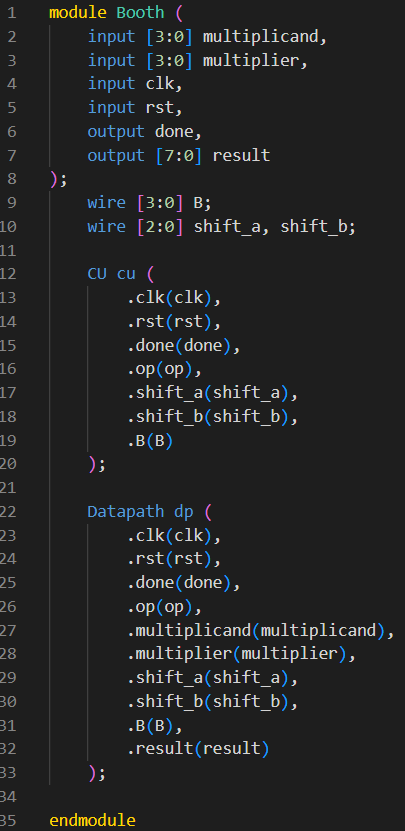
\includegraphics[width=0.6\textwidth]{Booth.png}
\end{figure}

\section{شبیه‌سازی و بررسی عملکرد ضرب‌کننده}
برای بررسی عملکرد ماژول اصلی یک ماژول تست برای آن مینویسیم.

\begin{figure}[H]
    \centering
    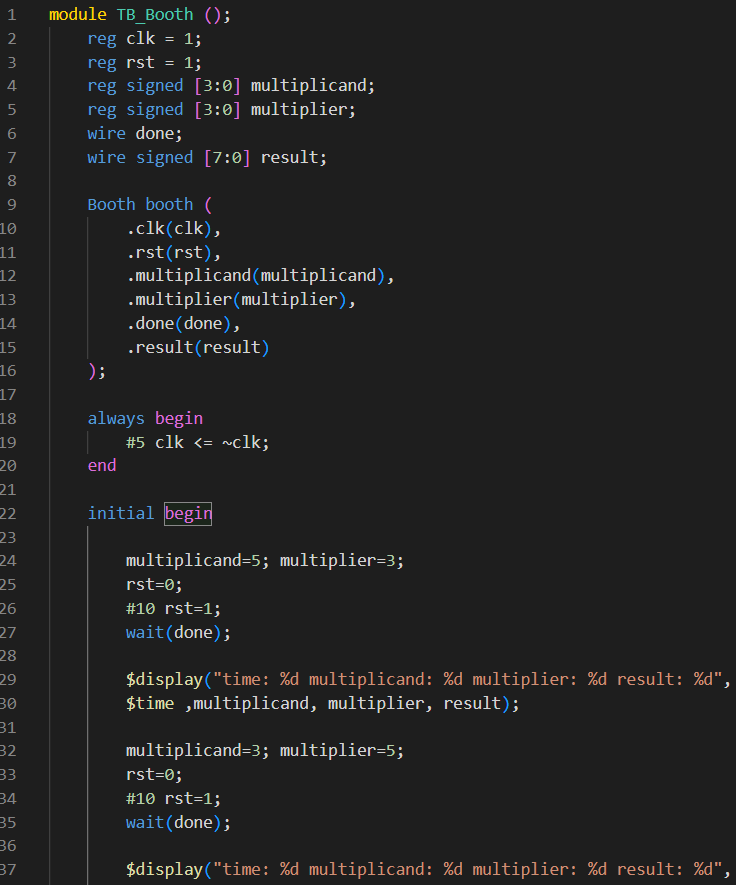
\includegraphics[width=0.85\textwidth]{TB_Booth1.png}
\end{figure}

\begin{figure}[H]
    \centering
    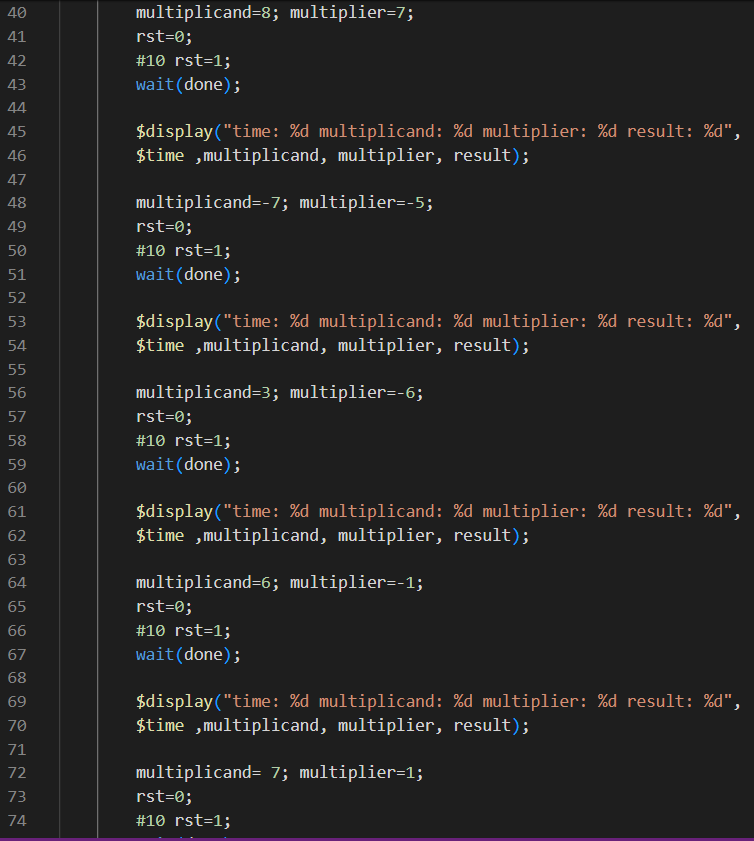
\includegraphics[width=0.7\textwidth]{TB_Booth2.png}
\end{figure}

\begin{figure}[H]
    \centering
    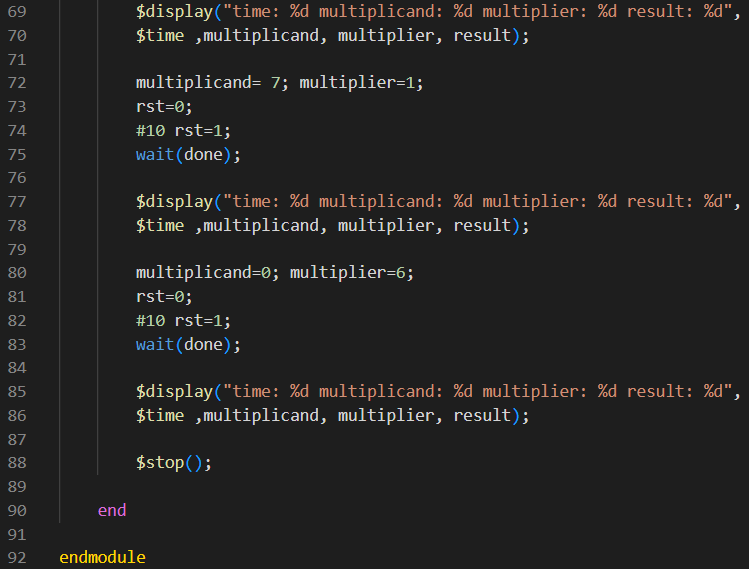
\includegraphics[width=0.7\textwidth]{TB_Booth3.png}
\end{figure}

حاصل شبیه‌سازی ماژول بالا را در شکل‌های زیر میتوانید مشاهده کنید.

\begin{figure}[H]
    \centering
    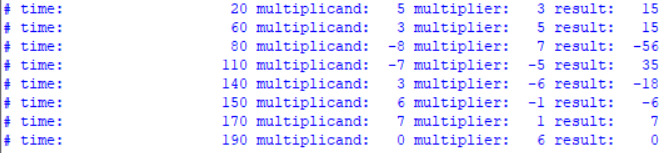
\includegraphics[width=\textwidth]{Res1.png}
\end{figure}

\begin{figure}[H]
    \centering
    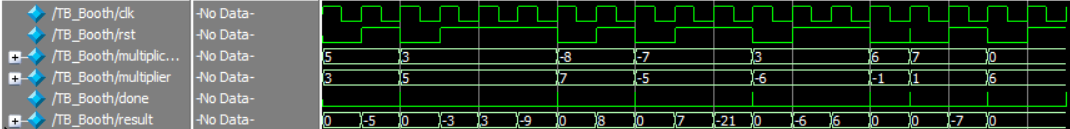
\includegraphics[width=\textwidth]{Res2.png}
\end{figure}

\end{document}